\documentclass[12pt,letterpaper]{article}
\usepackage[utf8]{inputenc}
\usepackage[spanish]{babel}
\usepackage{graphicx}
\usepackage[left=2cm,right=2cm,top=2cm,bottom=2cm]{geometry}
\usepackage{graphicx} % figuras
% \usepackage{subfigure} % subfiguras
\usepackage{float} % para usar [H]
\usepackage{amsmath}
%\usepackage{txfonts}
\usepackage{stackrel} 
\usepackage{multirow}
\usepackage{enumerate} % enumerados
\renewcommand{\labelitemi}{$-$}
\renewcommand{\labelitemii}{$\cdot$}
% \author{}
% \title{Caratula}
\begin{document}

% Fancy Header and Footer
% \usepackage{fancyhdr}
% \pagestyle{fancy}
% \cfoot{}
% \rfoot{\thepage}
%

% \usepackage[hidelinks]{hyperref} % CREA HYPERVINCULOS EN INDICE

% \author{}
\title{Caratula}

\begin{titlepage}
\begin{center}
\large{UNIVERSIDAD PRIVADA-DE-TACNA}\\
\vspace*{-0.025in}
\begin{figure}[htb]
\begin{center}

\includegraphics[width=8cm]{./Imagenes/logo}
\end{center}
\end{figure}
\vspace*{0.15in}
INGENIERIA DE SISTEMAS  \\

\vspace*{0.5in}
\begin{large}
TITULO:\\
\end{large}

\vspace*{0.1in}
\begin{Large}
\textbf{INFORME DE LABORATORIO No 02}\\
\end{Large}

\vspace*{0.3in}
\begin{Large}
\textbf{CURSO:} \\
\end{Large}

\vspace*{0.1in}
\begin{large}
INTELIGENCIA DE NEGOCIOS\\
\end{large}

\vspace*{0.3in}
\begin{Large}
\textbf{DOCENTE(ING):} \\
\end{Large}

\vspace*{0.1in}
\begin{large}
 Patrick Cuadros Quiroga\\
\end{large}

\vspace*{0.2in}
\vspace*{0.1in}
\begin{large}
Estudiante: \\ 
Sharon Sosa Bedoya          (2016054460) \\
\end{large}
\end{center}

\end{titlepage}


\tableofcontents % INDICE
\thispagestyle{empty} % INDICE SIN NUMERO
\newpage
\setcounter{page}{1} % REINICIAR CONTADOR DE PAGINAS DESPUES DEL INDICE

\section{INFORMACIÓN GENERAL} 

\begin{itemize}
\subsection{Objetivos:}
	\item Conocer los pasos sobre como realizar una graficos mediante una base de datos en PowerBi.
\subsection{Equipos, materiales, programas y recursos utilizados:}
	\item Windows 10 64bit: Pro, Enterprise o Education, con al menos 4GB de RAM.
	\item Base de datos AdventureWorksLT2016 o superior
	\item Tener los archivos de recursos del laboratorio.
	\item PowerBi Desktop
	\item Microsoft SQL Server 2017 o superior
	\item Tener una cuenta Microsoft registrada en el Portal de Power Bi

\end{itemize}

\section{PROCEDIMIENTO} 

\begin{itemize}
\subsection{Ejercicio 1: Conectando a Power BI a datos}
	\subsubsection{Parte 1: Conectar a datos existentes }

		\item Para realizar los gráficos en PowerBi Desktop primero debemos conectarnos con nuestra base de datos, que ya tiene que tener la base de datos "AdventureWorksLT2016".  Tambien tenemos que tener los archivos de "LabExcercise1.sql" donde se encuentra las Task para cargar los datos en PowerBi. \\Abrimos nuestro PowerBi desktop y procedemos a realizar la conexión a SQL server.
		\begin{figure}[h]
		\begin{center}
		\fbox{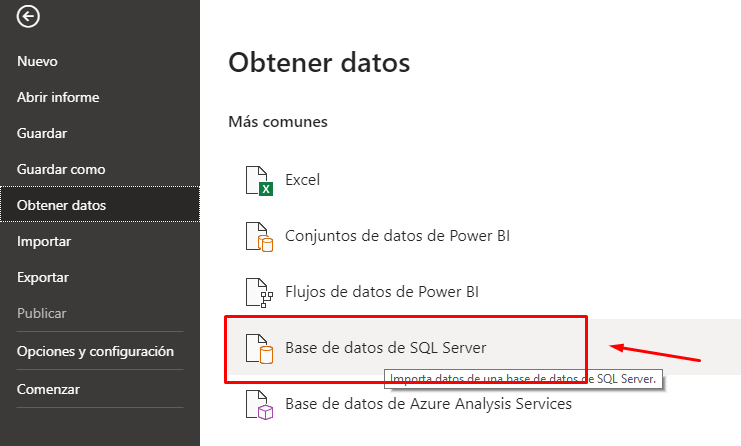
\includegraphics[width=9cm]{./Imagenes/tarea1}}
		\end{center}
		\end{figure}
		\begin{figure}[h]
		\begin{center}
		\fbox{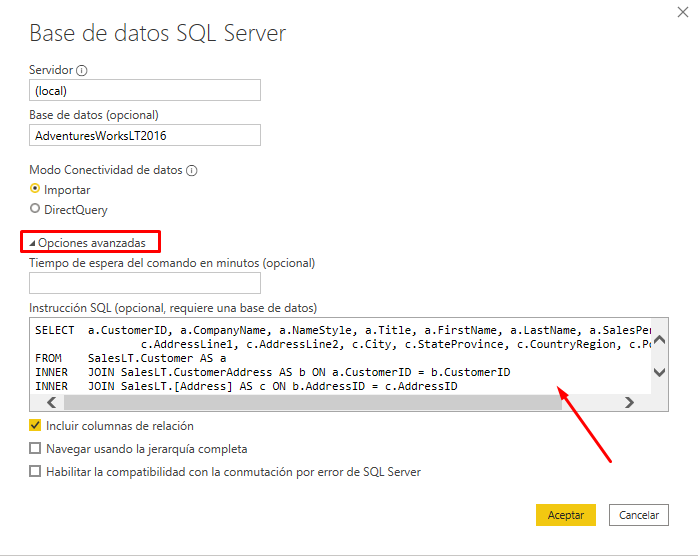
\includegraphics[width=12cm]{./Imagenes/tarea1_1}}
		\end{center}
		\end{figure}
		
\clearpage
		\begin{figure}[h]
		\begin{center}
		\fbox{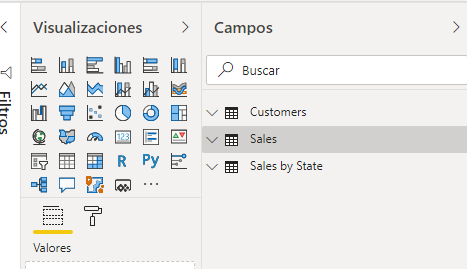
\includegraphics[width=11cm]{./Imagenes/tarea1_3}}
		\end{center}
		\end{figure}

		\item Una vez terminado de cargas los datos que necesitaremos, podremos visualizarlo en el panel lateral derecho de nombre "Campos".	
     \subsubsection{Parte 2: Graficar Datos }
	\item Los datos de cada tabla en la pestaña de "Campos" se va a configurar algunos datos. como el asignarle una categoria a un campo y la creacion de nuevas columnas de datos con los campos que ya tenemos.
\begin{figure}[h]
		\begin{center}
		\fbox{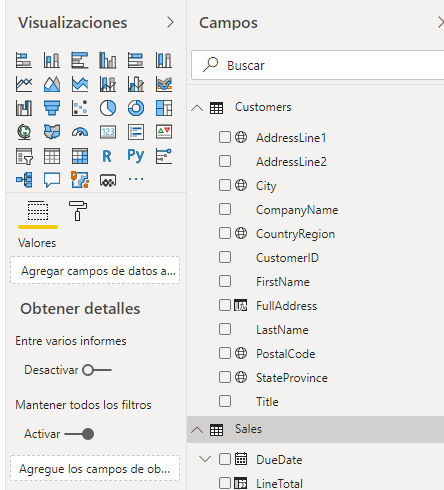
\includegraphics[width=9cm]{./Imagenes/tarea1_2}}
		\end{center}
		\end{figure}
\clearpage
\subsection{Ejercicio 2: : Adicionar Gráficos al Reporte}
	\item En la parte 2 realizaremos los gráficos con la información de la base de datos que seleccionamos. Utilizaremos del panel de Visualizaciones los diferentes gráficos que nos ofrecen.

\begin{itemize}
	\item{\textbf{1. Cantidad de Ventas del personal: }} Gráfico de Columna Apilada que nos muestra el reporte de la cantidad de ventas de cada personal de ventas.
	\item {\textbf{2. Número de Empleados por especialidad: }}En el gráfico de Pie, muestra los la cantidad de empleados que tiene la empresa según su especialidad.
	\item {\textbf{3. Top 10 Productos vendidos: }}El gráfico de Donut, muestra el top 10 de los productos más vendidos. Podremos visualizarlo representados en los diferentes colores en el gráfico.
	\item {\textbf{4. Ventas Anuales y Beneficios Anuales: }}En el segundo gráfico de Columna Apilada podremos visualizar la cantidad de ventas anuales y los beneficios que ha traido. 
	\end{itemize}

\begin{figure}[h]
	\begin{center}
	\fbox{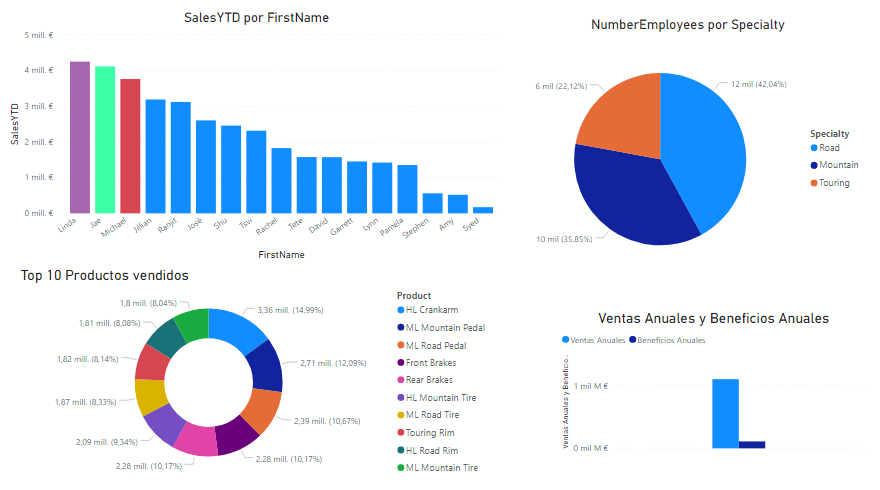
\includegraphics[width=15cm]{./Imagenes/tarea2}}
	\end{center}
	\end{figure}
		
\clearpage

\subsection{Parte 3: Publicar el reporte en el portal de Power BI}
	\item Cuando los gráficos esten listos, seleccionamos la opción de "Publicar" que nos ofrece PowerBi y poder subirlo a nuestra "Área de Trabajo". Cuando damos a "Aceptar" el archivo se irá subiendo a nuestra cuenta.

\begin{figure}[h]
	\begin{center}
	\fbox{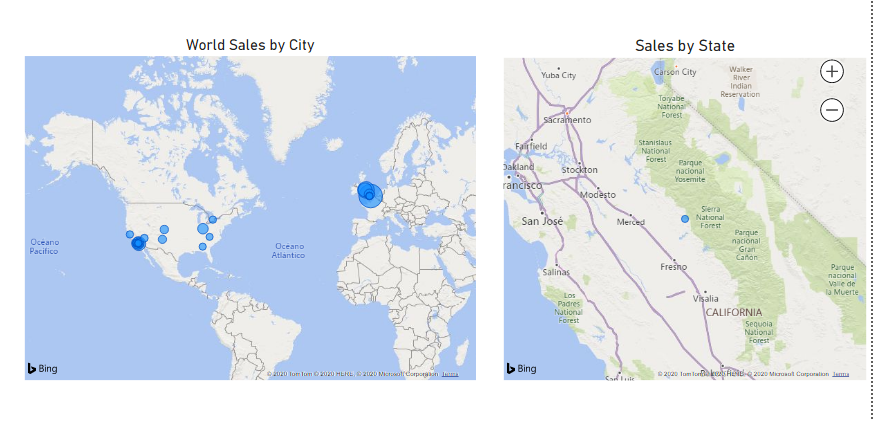
\includegraphics[width=11cm]{./Imagenes/tarea3}}
	\end{center}
	\end{figure}

\item Una vez se haya terminado de subir, abrimos nuestra cuenta desde la página web de Microsoft PowerBi y podremos visualizar nuestro trabajo ahí.

\begin{figure}[h]
	\begin{center}
	\fbox{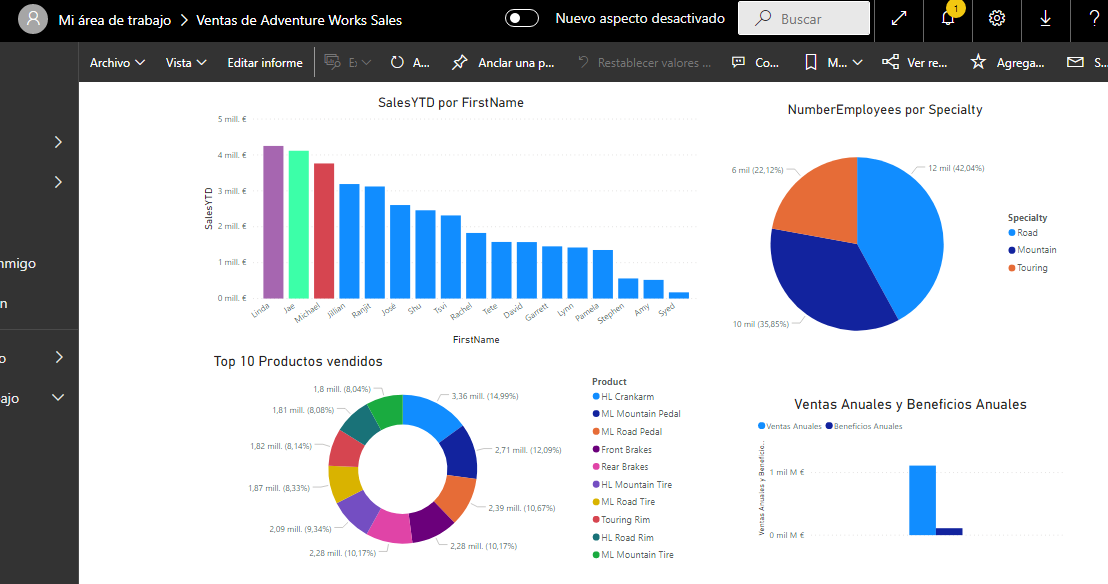
\includegraphics[width=14cm]{./Imagenes/tarea3_1}}
	\end{center}
	\end{figure}

\end{itemize}
		
\section{CONCLUSIONES}
\begin{itemize}
\item Business Intelligence y sus herramientas como PowerBi se ha posicionado como líder en este campo en solo unos años, e incluso si hay otras soluciones avanzadas, Microsoft ha invertido tantos recursos en el desarrollo de Power BI y su posición privilegiada en el mercado esta creciendo cada vez más.
\item Te permite extraer información importante para una amplia gama de escenarios, también permite ptimizar, limpiar, transformar y combinar datos de múltiples orígenes. Analizar en profundidad los datos y encontrar patrones.
\item Se puede crear diversos informes sorprendentes con los gráficos que ofrece para la visualización de los datos de forma interactiva.
\end{itemize}

\newpage


\end{document}
